\documentclass[11pt]{article}
\usepackage{fullpage}
\usepackage{authblk}
\usepackage{graphicx}
\usepackage{subfig}
\usepackage{amsmath}
\usepackage{amsfonts}
\usepackage{amssymb}
\usepackage{amsthm}
\usepackage{mathrsfs}
\usepackage{enumitem}
\usepackage[ruled,vlined]{algorithm2e}

\newtheorem{theorem}{Theorem}[section]
\newtheorem{lemma}[theorem]{Lemma}
\newtheorem{claim}[theorem]{Claim}
\newtheorem{corollary}[theorem]{Corollary}
\newtheorem{proposition}[theorem]{Proposition}
\newtheorem{definition}[theorem]{Definition}
\newtheorem{remark}[theorem]{Remark}
\newtheorem{assumption}[theorem]{Assumption}
\newtheorem{hypothesis}[theorem]{Hypothesis}
\newtheorem{observation}[theorem]{Observation}

\makeatletter
\renewcommand\section{%
  \@startsection{section}{1}
                {\z@}%
                {-3.5ex \@plus -1ex \@minus -.2ex}%
                {2.3ex \@plus.2ex}%
                {\large\bfseries}% 11pt
}
\renewcommand\subsection{%
  \@startsection{subsection}{2}
                {\z@}%
                {-3.25ex\@plus -1ex \@minus -.2ex}%
                {1sp}% No space after subsections
                {\normalsize\bfseries}% normal size, boldface
}
\renewcommand\subsubsection{%
  \@startsection{subsubsection}{3}
                {\z@}%
                {-3.25ex\@plus -1ex \@minus -.2ex}%
                {1sp}% No space after subsubsections
                {\normalfont\normalsize}% normal size, medium
}
\makeatother
\marginparwidth 0pt \oddsidemargin 0pt \evensidemargin 0pt
\topmargin 30pt \textheight 21.0 truecm \textwidth 16.0 truecm

\title{\bf Packing Feedback Arc Sets in Reducible Flow Graphs}
\author{Han Xiao}

\affil{Department of Mathematics, The University of Hong Kong,

Hong Kong, China

{\tt hxiao.math@connect.hku.hk}}

\begin{document}
 \date{}
\maketitle
%\thispagestyle{empty}

\begin{abstract}
In this paper we establish a min-max relation in arc-weighted reducible flow graphs. In particular, we prove that the maximum cardinality of feedback arc set packings equals the minimum total weight of cycles.  We also present an $O(n^2 m)$ algorithm for finding a maximum feedback arc set packing in reducible flow graphs.
\end{abstract}

\noindent{\bf Keywords.}\quad Min-max relation, feedback arc set, packing, reducible flow graph, algorithm


\openup 1.2\jot


\section{Introduction}
\label{intro}

A reducible flow graph is a special flow graph which corresponds to the flowchart of computer programs via structured programming. As mentioned by Hecht \cite{Hech}, the ``divide-and-conquer'' approach applies to reducible flow graphs, which makes the analysis easier on such graphs. Reducible flow graphs also occur frequently in practice. Statistics suggest that most flow graphs associated with computer programs are reducible flow graphs. Therefore, reducible flow graphs have attracted many research efforts over the past few decades. Various characterizations of reducible flow graphs can be found in the work of Hecht and Ullman \cite{HecU1}. The first efficient algorithm for recognizing reducible flow graphs was given by Hopcroft and Ullman \cite{HopU}. Based on their work, Tarjan \cite{Tarj} derived a more efficient algorithm for testing flow graphs reducibility. 

In this paper, by a cycle (\emph{resp.} path) in a digraph we mean a directed one. A digraph is called \emph{acyclic} if it contains no cycles, and is abbreviated a \emph{DAG} (directed acyclic graph). Let $G=(V,A)$ be a digraph with a nonnegative integral function $w$ defined on arcs in $A$. A set $F\subseteq A$ is a \emph{feedback arc set} (\emph{FAS}) for $G$ if $G^\prime=(V,A\backslash F)$ is acyclic. Let $H=(A,\mathcal{C})$ be a hypergraph whose vertex set is the arc set of $G$ and edges are the arc sets of cycles in $G$. A collection (with repetition allowed) $\mathcal{C}^\prime$ of edges in $H$ is called a \emph{cycle packing} if each arc $a\in A$ occurs at most $w(a)$ times in cycles of $\mathcal{C}^\prime$. A \emph{transversal} of a hypergraph is a subset of its vertex set which intersects each edge of the hypergraph. Note that a transversal of $H=(A,\mathcal{C})$ is a feedback arc set of $G$. Let $\nu_w$ denote the maximum cardinality of cycle packings and $\tau_w$ denote the minimum weight of feedback arc sets. It is easy to prove that $\nu_w\leq\tau_w$. When equality $\nu_w=\tau_w$ holds for all nonnegative integral function $w$, the hypergraph $H$ is said to satisfy the min-max relation and the graph $G$ is said to be \emph{cycle Mengerian} (\emph{CM}). Ramachandran \cite{Rama1} gave an $O(n^2m\log(n^2 / m))$ algorithm for finding a minimum weight feedback arc set in arc-weighted reducible graphs. She \cite{Rama2} also established a conjecture of Frank and Gyarfas \cite{FraG} by showing that the minimum cardinality of feedback arc sets is equal to the maximum cardinality of cycle packings  in unweighted reducible flow graphs. Her proof yielded an $O(\min\{mn^{5/3},m^2\})$ algorithm for finding a maximum collection of arc disjoint cycles. Chen and Zang \cite{CheZ} pointed out that although Ramachandran's proof \cite{Rama2} was intended for unweighted reducible flow graphs, it could be adapted to handle the weighted case. Based on Ramachandran's work \cite{Rama1,Rama2}, Chen and Zang \cite{CheZ} proved that every reducible flow graph is CM. They also reduced the time complexity of finding a maximum cycle packing in weighted reducible flow graphs to $O(n^2 m\log(n^2/m))$  by avoiding using augmenting path method for finding the maximum flow as a subroutine in their algorithm. 

A \emph{clutter} is a hypergraph no edge of which is contained in another. Note that hypergraph $H=(A,\mathcal{C})$ is a clutter. The hypergraph $H^\perp=(A,\mathcal{F})$ is called the \emph{blocker} of $H$, where vertex set of $H^\perp$ is the arc set of $G$ and edges are feedback arc sets in $G$. Analogous to the definition of cycle packing, we call a collection (with repetition allowed) $\mathcal{F}^\prime$ of edges in $H^\perp$ a \emph{feedback arc set packing} if each arc $a$ occurs at most $w(a)$ times in feedback arc sets of $\mathcal{F}^\prime$. Note that a transversal of $H^\perp$ is a cycle in $G$. Let $\lambda_w$ denote the maximum cardinality of feedback arc set packings and $\mu_w$ denote the minimum weight of cycles. Obviously, $\lambda_w\leq\mu_w$. When equality $\lambda_w=\mu_w$ holds for all nonnegative integral function $w$, the hypergraph $H^\perp$ is said to satisfy the min-max relation and the graph $G$ is said to be \emph{feedback arc set Mengerian} (\emph{FASM}). It has been proved that hypergraph $H=(A,\mathcal{C})$ derived from reducible flow graph $G=(V,A)$ satisfies the min-max relation. Hence every reducible flow graph is CM. A natural question is whether the blocker $H^\perp=(A,\mathcal{F})$ of hypergraph $H$ satisfies the min-max relation as well. The main contribution of this paper is twofold. First, we give an affirmative answer to this question, hence every reducible flow graph is FASM. Second, we present an $O(n^2 m)$ algorithm for finding a maximum feedback arc set packing in reducible flow graphs. Our result relies heavily on the structural analysis for reducible flow graphs of Ramachandran's work \cite{Rama1,Rama2}.

The remainder of this paper is organized as follows. In section 2, we introduce some preliminary knowledge on reducible flow graphs. In section 3, we first prove that every reducible flow graph is FASM, then we present our algorithm and establish its correctness.

\section{Preliminaries}
\label{prel}

A \emph{flow graph} is a digraph with a root such that the root reaches all other vertices via paths.
Let $G=(V,A;r)$ be a flow graph with root $r$. 
A \emph{DAG} of $G$ is a maximal acyclic subgraph of $G$ which remains a flow graph with root $r$. We call $G$ \emph{reducible} if the DAG of $G$ is unique. A DAG of $G$ obtained from a depth-first spanning tree rooted at $r$ by adding a maximal subset of arc set $A$ is called a \emph{DFS DAG} of $G$.
For $u,v\in V$, we say $u$ \emph{dominates} $v$ if every $r-v$ path passes through $u$. Clearly, every vertex dominates itself. For a subgraph $G'$ of $G$, a vertex $v$ of $G'$ is called an \emph{entry vertex} if $v=r$ or there is an arc $(u,v)$ of $G$ with $u$ outside $G'$.  Observe that arcs in a reducible flow graph can be uniquely partitioned into the \emph{forward} (or \emph{DAG}) \emph{arc} set and the \emph{back arc} set.

Following are some useful characterizations of reducible flow graphs.
\begin{theorem}
\label{thm:1}
Let $G=(V,A;r)$ be a flow graph and let $D$ be a DFS DAG of $G$. Then the following statements are equivalent:
\begin{enumerate}[label=\emph{(}\alph*\emph{)}]
  \item $G$ is a reducible flow graph.
  \item $F$ is the unique obstruction for the transitive closure of $G$ (see Figure \ref{fig:1}).
  \item $D$ is the unique DAG of $G$.
  \item The arc set $A$ can be partitioned into $A_1$ and $A_2$ such that $(V,A_1;r)$ is a DAG of $G$ and $u$ dominates $v$ in $G$ for each arc $(v,u)$ in $A_2$.
  \item Every cycle $C$ in $G$ contains exactly one back arc $a\in A\backslash A(D)$. Moreover, the head of back arc $a\in A\backslash A(D)$ is the entry vertex of $C$ which dominates other vertices on $C$.
\end{enumerate}
\end{theorem}

\begin{figure}
\centering
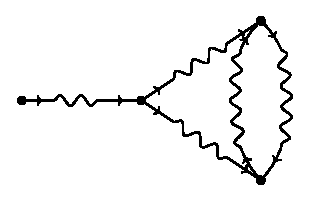
\includegraphics[scale=.55]{FASPacking-fig1.eps}
\caption{The obstruction $F$}
\label{fig:1}
\end{figure}

\begin{proof}
The equivalence of $(a)-(d)$ can be found in the work of  Hecht and Ullman \cite{HecU1,HecU2}. The implication $(a)\Rightarrow (e)$ is proved by Shamir \cite{Sham} and the converse direction $(e)\Rightarrow (a)$ is discovered by Chen and Zang \cite{CheZ}.
\end{proof}

Following are some notations introduced by Hecht, Ullman \cite{HecU1, HecU2} and Ramachandran \cite{Rama1,Rama2}. Let $V_h$ denote the set of the head of all back arcs in $G$. Let $T_h$ denote the \emph{head dominator tree} of $G$ which demonstrates the domination relation on $V_h\cup \{r\}$: the descendants of vertex $u$ in $T_h$ are precisely the vertices in $V_h$ dominated by $u$ in $G$. For $u\in V_h\cup\{r\}$, $(u_1,v_1),(u_2,v_2),\ldots,(u_k,v_k)$ represent all the back arcs in $G$ whose head is dominated by $u$. Let $V_u$ denote the \emph{dominated back arc vertex set} of $u$ which consists of all the vertices in $V$ lying on some DAG path from $u$ to $u_i$, for $1\leq i\leq k$. Ramachandran \cite{Rama1,Rama2} proved that $u$ dominates all vertices in $V_u$. And $G_s(V_u)$ denotes the subgraph of $G$ induced by $V_u$ (see Figure \ref{fig:2}).

\begin{figure}
    \centering
    \subfloat[$G=(V,A;v_1)$]{
    \begin{minipage}[t]{0.33\linewidth}
          \centering
          \includegraphics[scale=.38]{FASPacking-fig2a.eps}
          \label{fig:2a}
    \end{minipage}}
    \subfloat[$T_h$]{
     \begin{minipage}[t]{0.33\linewidth} 
          \centering
          \includegraphics[scale=.38]{FASPacking-fig2b.eps}
          \label{fig:2b}
    \end{minipage}}
    \subfloat[$G_s(V_{v_4})$]{
    \begin{minipage}[t]{0.33\linewidth} 
          \centering
          \includegraphics[scale=.38]{FASPacking-fig2c.eps}
          \label{fig:2c}
    \end{minipage}}  
    \caption{A reducible flow graph $G$ and its $T_h$, $G_s(V_{v_4})$}
     \label{fig:2}
 \end{figure}

The following properties of dominated back arc vertex sets were established by Chen and Zang \cite{CheZ}.

\begin{theorem}
\label{thm:2}
Let $G=(V,A;r)$ be a reducible flow graph and let $u$, $v$ be two vertices in $V_h\cup\{r\}$. Then the following statements hold:
\begin{enumerate}[label=\emph{(}\alph*\emph{)}]
  \item $G_s(V_u)$ is a reducible flow graph rooted at $u$.
  \item $u$ is the unique entry vertex of $G_s(V_u)$ in $G$.
  \item If $G_s(V_u)$ and $G_s(V_v)$ have a common vertex, then either $u$ dominates $v$ or $v$ dominates $u$.
\end{enumerate}
\end{theorem}

\section{Maximum feedback arc set packings in reducible flow graphs}
\label{sec:3}

\subsection{Min-max relation}
\label{sec:4}

Let $G=(V,A;r)$ be a reducible flow graph with a nonnegative integral weight $w$ on arcs in $G$. We construct a network $N(r,t)$ from $G$ as follows. Add a new vertex $t$. For $v\in V_h$, make a copy $v'$, redirect back arcs from $v$ to $v'$ and connect $v'$ to $t$ by a \emph{newly added arc} $(v^\prime,t)$ (see Figure 3).
We also define a length function $l$ on arcs in $N$ from the weight function $w$ on arcs in $G$: first, set $l(a)=w(a^\prime)$ for each arc $a\in A(N)$ that corresponds to arc $a^\prime\in A$; then, for each newly added arc $a=(v^\prime,t)$ in $A(N)$, set $l(a)=d-d(v)$, where $d(v)$ is the distance from $r$ to $v$ in $N$ and $d:=\max_{v\in V_h} d(v)$ is the largest distance from $r$ to every vertex in $V_h$. Obviously, $l(a)\geq 0$ for all $a\in A(N)$. In network $N(r,t)$, the set of all vertices at distance less than $i$ from $r$ is denoted by $U_i$ and the set of all outgoing arcs of set $U_i$ is denoted by $\partial^+(U_i)$.

\begin{figure}
    \centering
    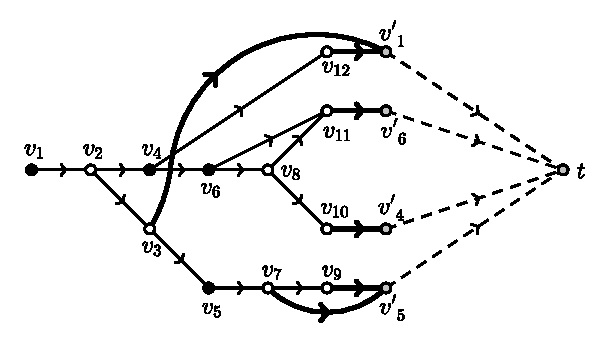
\includegraphics[scale=0.8]{FASPacking-fig3.eps}
    \caption{$N(v_1,t)$ constructed from $G=(V,A;v_1)$}
     \label{fig:3}
 \end{figure}

\begin{lemma}
\label{lem:2}
For $v\in V_h$, the following statements hold:
\begin{enumerate}[label=\emph{(}\alph*\emph{)}]
  \item Every $r-v'$ path goes through $v$.
  \item There is a one to one correspondence between cycles whose head of the back arc is $v$ in $G$ and $v-t$ paths going through $v^\prime$ in $N(r,t)$. 
  \item The length of the shortest $r-t$ paths going through $v^\prime$ is $d+d(v,v^\prime)$.
\end{enumerate}
\end{lemma}
\begin{proof}
By Theorem \ref{thm:2}, $v$ is the unique entry vertex of $G_s(V_v)$. Then by the construction of $N(r,t)$, $(a)$ and $(b)$ follow directly.

Since any part of a shortest path is also a shortest path, so the length of the shortest $r-t$ paths going through $v^\prime$ is $d(v)+d(v,v^\prime)+d(v^\prime,t)=d(v)+d(v,v^\prime)+d-d(v)=d+d(v,v^\prime)$.
\end{proof}

Let $K$ denote the minimum total weight of cycles in $G$. By Lemma \ref{lem:2}, $d(t)=\min_{v\in V_h}\{d+d(v,v^\prime)\}=d+K$, implying that the total number of $r-t$ cuts $\partial^+(U_i)$ in $N$ is $d+K$.
For $v\in V_h$, let $C_v$ denote the collection of all cycles in $G$ whose head of the back arc is $v$. With a slight abuse of notation, we call $\partial^+(U_i)$ is a \emph{FAS} of $C_v$ if it cuts off all $v-v'$ paths in $N$. We call $\partial^+(U_i)$ a \emph{quasi-FAS} of $C_v$ if it cuts off all $v-t$ paths in $N$. Let $\mathcal{C}$ be the collection of $C_v$ for $v\in S\subseteq V_h$. We call $\partial^+(U_i)$ a \emph{quasi-FAS} of $\mathcal{C}$ if $\partial^+(U_i)$ is a quasi-FAS for $C_v\in\mathcal{C}$. By Lemma \ref{lem:2}, it is easy to see that $\partial^+(U_i)$ is a FAS of $C_v$ if $d(v)<i\leq \min\{d(t),d(v^\prime)\}$, a quasi-FAS of $C_v$ if $d(v) <i\leq d(t)$, a quasi-FAS of $\mathcal{C}$ if $\max_{v:C_v\in \mathcal{C}}d(v)<i\leq d(t)$.

 As we shall see, initializing $\mathcal{C}$ with $\{C_v: v\in V_h\}$, recursively choosing some quasi-FAS $\partial^+(U_i)$ of current $\mathcal{C}$ and deleting $C_v$ that are broken by $\partial^+(U_i)$ from $\mathcal{C}$ always end with an empty set $\mathcal{C}$.
 When $\mathcal{C}$ becomes empty, the union of all the chosen quasi-FASs cuts off all $v-v'$ paths for $v\in V_h$, which yields a FAS of $G$ naturally.
 For clarity, we call an execution of choosing a quasi-FAS of $\mathcal{C}$ and deleting $C_v$ that are broken from $\mathcal{C}$ an \emph{iteration} and call the process of constructing a FAS of $G$ a \emph{stage}.

To make sure each stage ends properly, it suffices to show that in each iteration, the chosen quasi-FAS of current $\mathcal{C}$ is a FAS of some $C_v\in\mathcal{C}$. Notice that in the worst case, each $C_v$ in $\mathcal{C}$ needs a FAS. Hence we turn to show there are enough FASs of $C_v$ for $v\in V_h$ throughout a stage.

\begin{lemma} 
\label{lem:3}
At each stage, initialize $\mathcal{C}$ with $\{C_v:v\in V_h\}$, recursively choose the first available\footnote{`First available' here refers to the unused $r-t$ cut $\partial^+(U_i)$ with the least index $i$.} quasi-FAS of $\mathcal{C}$ and delete $C_v$ that are broken from $\mathcal{C}$, then $\mathcal{C}$ becomes empty after finite iterations. Moreover, at the end of stage $k$, the number of available FAS of $C_v$ is at least $K-k$ for $v\in V_h$.
\end{lemma}

Our proof of Lemma \ref{lem:3} is based on the following observation. 

\begin{lemma}
\label{lem:4} 
In each iteration of a stage, let $\mathcal{C}'$ be a subset of $\mathcal{C}$ such that the first available quasi-FAS of $\mathcal{C}$ is the first available FAS of $C_v$ for $C_v \in\mathcal{C}^\prime$. When $\mathcal{C}'$ is not empty,  there exists a $C_u\in \mathcal{C}^\prime$ such that the number of available FAS of $C_u$ decreases by precisely one in this stage.
\end{lemma}

\begin{proof}
At the end of each iteration, all cycle classes in $\mathcal{C}^\prime$ will be deleted from $\mathcal{C}$. Hence no quasi-FAS of $\mathcal{C}'$ is chosen in the succeeding iterations of this stage. Assume to the contrary that there is an FAS for $C_v\in\mathcal{C}'$ chosen before this iteration, then the first available quasi-FAS of $\mathcal{C}$ no longer depends on $\mathcal{C}'$, as $\mathcal{C}^\prime$ is deleted from $\mathcal{C}$ before this iteration, a contradiction.
\end{proof}

Notice that each $r-t$ cut $\partial^+(U_i)$ can only be used once in an FAS packing. Therefore, at the end of each stage, we reduce the value of $l(a)$ by one for $a\in \partial^+(U_i)$ if $\partial^+(U_i)$ is chosen during this stage. The distance $d(v)$ for $v\in V(N)$ with respect to the latest length function $l$ provides some useful information in each stage. For $v\in V_h$, $\min\{d(t),d(v^\prime)\}-d(v)$ is the number of available FASs of $C_v$. Besides, the first available quasi-FAS of $\mathcal{C}$ in each iteration of a stage is exactly the first available quasi-FAS of some $C_v$ with the largest $d(v)$ in $\mathcal{C}$.

Now we are ready to present a proof of our key lemma.

\begin{proof}[Proof of Lemma \ref{lem:3}]
We apply induction on the number of stages.

Observe that the initial state, viewed as stage 0, automatically satisfies the induction hypothesis. Therefore, the proof of basis and the proof of induction step are essentially the same. So we proceed to the induction step. Suppose the statement in Lemma \ref{lem:3} holds for stage $k\geq 0$. We aim to establish the statement for stage $k+1$.

We initialize $\mathcal{C}$ with $\{C_v:v\in V_h\}$. By induction hypothesis,  the number of available FAS of $C_v$ for $v\in V_h$ is at least $K-k>0$ at the beginning of stage $k+1$. Consider an arbitrary $C_u$ in $\mathcal{C}$. Let $\partial^+(U_{i_\tau}),\dots,\partial^+(U_{i_1})$ be all the FASs of $C_u$ chosen as the first available quasi-FAS of a series of nested sets $\mathcal{C}^{(\tau)}\subset\dots\subset\mathcal{C}^{(1)}:=\mathcal{C}$ respectively in stage $k+1$. If $\tau=1$, the number of available FAS of $C_u$ decreases by one, which is trivial. So assume $\tau\geq 2$. Let $u_j\in V_h$ be a vertex with the largest $d(v)$ among all $C_v\in \mathcal{C}^{(j)}$ for $j=\tau,\dots,1$. Without loss of generality, assume $C_{u_j}$ is a cycle class in $\mathcal{C}^{(j)}$ whose number of available FASs decreases by one in this stage. By Lemma \ref{lem:4}, such $C_{u_j}$ exists. By induction hypothesis, the first available quasi-FAS $\partial^+(U_{i_j})$ of $\mathcal{C}^{(j)}$ is also the first available FAS of $C_{u_j}\in \mathcal{C}^{(j)}$. It follows that $d(u)\leq d(u_\tau)< d(u^\prime_\tau)\leq\dots\leq d(u_1)< \min\{d(t),d(u^\prime)\}$. Clearly, $C_u$ is not the cycle class with the least number of available FASs in $\{C_v:v\in V_h\}$, since $\min\{d(t),d(u^\prime)\}-d(u)> d(u_\tau^\prime)-d(u_\tau)$. Moreover, by Lemma \ref{lem:4}, the number of available FASs of $C_{u_j}$ decreases by one in this stage. It follows that the number of available FASs of $C_u$ decreases by $\tau$, but is no less than $K-k-1$ at the end of stage $k+1$.

Therefore, there are available FASs of $C_v$ for $v\in V_h$ in each iteration of stage $k$ whenever $k\leq K$. Hence the first available quasi-FAS of $\mathcal{C}$ is always an available FAS of some $C_v\in \mathcal{C}$, implying the cardinality of $\mathcal{C}$ decreases in each iteration and the stage ends after finite iterations.
\end{proof}

By Lemma \ref{lem:3}, whenever $k\leq K$, stage $k$ returns an FAS of $G$ . Hence an FAS packing of cardinality $K$ is attained. Since $K$ is also the minimum total weight of cycles in $G$, the following theorem follows directly.

\begin{theorem}
\label{thm:4}
Every reducible flow graph is FASM.
\end{theorem}

\subsection{Algorithm and complexity}
\label{sec:5}
The constructive proof of Theorem \ref{thm:4} naturally yields an algorithm for finding a maximum FAS packing in reducible flow graphs. However, regardless of other operations, one needs to repeat stage $K$ times to get a maximum FAS packing, which makes the algorithm pseudo-polynomial. Observe that consecutive stages might return the same FAS because chosen quasi-FASs in consecutive stages might be the same. Hence a natural idea is to merge stages returning the same FAS into one.  
Suppose we have merged the first $k-1$ stages returning the same FAS into $\kappa-1$ new STAGEs respectively and updated the length function $l$ accordingly. Now we are at stage $k$ which cannot be merged into STAGE $\kappa-1$. We initialize $\mathcal{C}$ with $\{C_v:v\in V_h\}$. Then we recursively choose the first available quasi-FAS of $\mathcal{C}$, delete $C_v$ from $\mathcal{C}$ that are broken, and update $d$ by $\max_{C_v\in\mathcal{C}} d(v)$. After $j\geq 0$ iterations, we arrive at a nonempty set $\mathcal{C}$. Clearly, $\partial^+(U_{d+1})$ is the first available quasi-FAS of $\mathcal{C}$. Observe that the following $\min_{(u,w)\in\partial^+(U_{d+1})}\{d(w)-d\}$ quasi-FASs of $\mathcal{C}$ including $\partial^+(U_{d+1})$ are actually the same arc set. If $\mathcal{C}$ occurs in succeeding stages, the same arc set might be chosen. Hence we introduce a parameter $\alpha$. In each iteration of stage $k$, we update $\alpha$ (initialized with a value large enough) by the smaller value of current $\alpha$ and $\min_{(u,w)\in\partial^+(U_{d+1})}\{d(w)-d\}$, where $\partial^+(U_{d+1})$ is the first available quasi-FAS of current $\mathcal{C}$. When $\mathcal{C}$ becomes empty, quasi-FASs chosen in the succeeding $\alpha$ stages including stage $k$ are the same. It follows that the succeeding $\alpha$ stages including stage $k$ give rise to the same FAS of $G$. Therefore, we merge these $\alpha$ stages including stage $k$ into new STAGE $\kappa$. Let $\mathcal{T}$ be the collection of all the chosen quasi-FASs of stage $k$. At the end of STAGE $\kappa$, instead of updating the length function $l$ separately, we reduce $l(a)$ by $\alpha$ for $a\in \partial^+(U_i)$ if $\partial^+(U_i)\in\mathcal{T}$.

The following lemma guarantees that, by making the biggest jump on stages in exchange for efficiency, our construction ends in $O(n)$ STAGEs, where $n$ is number of vertices in $G$.

\begin{lemma}
\label{lem:5}
By merging consecutive stages returning the same FAS into a new STAGE, the construction ends in $O(n)$ STAGEs, where $n$ is the number of vertices in the reducible flow graph.
\end{lemma}
\begin{proof}
At the beginning of our construction, we decompose $V(N)$ into at most $\lvert V(N)\rvert$ partitions according to the distance $d(v)$ with respect to initial length function $l$. At each STAGE, there exists a chosen quasi-FAS $S$ satisfying equality $\alpha=\min_{(u,w)\in S} d(w)-\max_{(u,w)\in S} d(u)$. At the end of this STAGE, the length of each arc in quasi-FAS $S$ decreases by $\alpha$. It follows that the vertex set of distance $\min_{(u,w)\in S} d(w)$ and the vertex set of distance $\max_{(u,w)\in S} d(u)$ merge into one vertex set of the same distance. Therefore, the number of decompositions decreases by at least one in each STAGE. After $O(\lvert V(N)\rvert)$ STAGEs, all vertices in $V(N)$ belong to the same distance class, implying the termination of our construction. By the construction of network $N$, $\lvert V(N)\rvert\leq 2n+1$. Hence the construction ends in $O(n)$ STAGEs.
\end{proof}
Now we are ready to present our algorithm (see Algorithm 1). 
\SetAlFnt{\small}
\begin{algorithm}[!ht]
  \SetAlgoLined
  \SetAlgoNoEnd
 %\DontPrintSemicolon
  \SetKwFunction{Augment}{Augment}
  \SetKwFunction{Update}{Update}
  \SetKwInOut{Input}{Input}\SetKwInOut{Output}{Output}
  \Input{An arc-weighted reducible flow graph $G=(V,A;r)$}
  \Output{A maximum FAS packing $\mathcal{F}$ of $G$}
  \BlankLine
  Construct $N(r,t)$ and define the length function $l$\; %\tcc*[r]{This step yields all $U_d$}
  $d\leftarrow \max_{v\in V_h}d(v)$\;
  $\mathcal{F}\leftarrow \emptyset$\;
  \While{$d< d(t)$}{
    $\mathcal{T}\leftarrow \emptyset$\;
    $F\leftarrow \emptyset$\;
    $\alpha\leftarrow d(t)$\;
    \Augment($\partial^+(U_{d+1})$)\;
    Delete newly added arcs in $F$ and replace remaining arcs by corresponding arcs in $G$\;
    $\mathcal{F}\leftarrow \mathcal{F}\cup \{(F,\alpha)\}$\;
    \Update($l$)\;
    Find $d(v)$ for $v\in V(N)$ with respect to the latest $l$\;
    $d\leftarrow \max_{v\in V_h} d(v)$\;
    }
  Return $\mathcal{F}$\;
  \BlankLine
  \SetKwProg{myproc}{procedure}{}{}
  \myproc{\Augment{$S$}}{
  $\mathcal{T}\leftarrow \mathcal{T}\cup\{S\}$\;
  $F\leftarrow F\cup S$\;
  $\alpha\leftarrow\min\{\alpha,\min_{(u,w)\in S}\{d(w)-d\}\}$\;
  \If{$\exists (v^\prime,t)\in S$}{
    $d\leftarrow \max_{(v^\prime,t)\in S} d(v)$\;
    \Augment($\partial^+(U_{d+1})$)\; 
    }
  }
  \myproc{\Update{$l$}}{
  \For{$T\in\mathcal{T}$}{
  \For{$a\in T$}{
  $l(a)\leftarrow l(a)-\alpha$\;
  }
  }
  }
  \caption{Max FAS Packing}
\end{algorithm} 

In our algorithm, we calculate $d(v)$ for $v\in V(N)$ with respect to the latest length function $l$ repeatedly. The following lemma ensures that this task can be done efficiently due to the special structure of $N$, a DAG.

\begin{lemma}
\label{lem:6}
All the single source shortest distances in an acyclic digraph $D=(V,A)$ can be found in $O(n+m)$, where $n=\lvert V \rvert$ and $m=\lvert A \rvert$.
\end{lemma}
\begin{proof}
Let $l:A\rightarrow \mathbb{R}$ be the length function defined on arcs of $D$ and $r\in V$ be the source given. Denote the distance of $v$ from $r$ by $d(v)$ for every $v\in V$. Initially, set $d(r)=0$ and $d(v)=+\infty$ for $v\in V\backslash \{r\}$, which takes $O(n)$ time. Then topologically sort all vertices and denote the ordering by $\pi$. This process can be finished in $O(m+n)$ time \cite{AhMO}. Visit every vertex $v$ in topological order and update $d(v)$ by $\min_{u:\pi(u)<\pi(v)}\{d(u)+l(u,v)\}$. This step returns the global shortest distance $d(v)$ because vertices behind $v$ in a topological order cannot be on any $r-v$ paths. Throughout the updating process, each arc is only visited once which requires $O(m)$ time. Hence the time complexity of finding all the shortest distances from $r$ is the same as the time complexity of topological sort, which is $O(m+n)$.
\end{proof}

\begin{theorem}
\label{thm:5}
In an arc-weighted reducible flow graph $G=(V,A;r)$, a maximum FAS packing can be found in $O(n^2 m)$ time, where $n=\lvert V \rvert$ and $m=\lvert A \rvert$.
\end{theorem}
\begin{proof}
By the construction of network $N(r,t)$, $\lvert V(N)\rvert\leq 2n+1$ and $\lvert A(N)\rvert\leq m+n$. It follows that $O(\lvert V(N)\rvert)=O(n)$. Since $G$ is connected, $O(\lvert A(N)\rvert)=O(m)$. Notice that the construction of network $N(r,t)$ involves calculating the shortest distance $d(v)$ for $v\in V_h$. By Lemma \ref{lem:6}, we can find all the distance $d(v)$ from $r$ in $O(m+n)=O(m)$ time. So the construction of network $N(r,t)$ requires $O(m)$ time. It is easy to see that all operations outside STAGEs take $O(m)$ time. By Lemma \ref{lem:5}, our algorithm ends in $O(n)$ STAGEs. It remains to show that the time complexity of each STAGE is $O(nm)$. Notice that each STAGE contains a recursive function $Augment(S)$ and a function $Update(l)$. Each invocation of function $Augment(S)$ in a STAGE decreases the number of newly added arcs in $S$ by at least one. So $Augment(S)$ in a STAGE ends in $O(n)$ invocations. Function $Augment(S)$ itself involves finding $\min_{(u,w)\in S}\{d(w)-d\}$ and $\max_{(v^\prime,t)\in S} d(v)$, both of which can be done in $O(n)$ time. So the complexity of function $Augment(S)$ in a STAGE is $O(n^2)$. As to function $Update(l)$, it requires $O(nm)$ time in a STAGE. Hence the time complexity of each STAGE is $O(nm)$. The theorem follows.
\end{proof}

\section*{Acknowledgments}
The author would like to thank Prof. Wenan Zang for his invaluable suggestions.

\bibliographystyle{spmpsci}
\bibliography{FASPacking}
\nocite{HecU2,Sham}

\end{document}
